% ==============================================================================
% CLEANED ms.tex (Optimized for XeLaTeX/Fira Fonts)
% - Consolidated preamble and ms.tex.
% - Removed all conflicting packages (lmodern, redundant font settings).
% - Uses Fira Sans/Mono/Math consistently.
% ==============================================================================

\documentclass[preview]{article}

% --- CORE FONT SETUP (Sans-Serif Headings, Serif Body, Professional Math) ---
\usepackage{fontspec}        
% Use Path=fonts/ to look inside the fonts folder
\setmainfont{FiraSans.ttf}[
    Path = fonts/,
    UprightFont = *-Regular,
    BoldFont = *-Bold,
    ItalicFont = *-Italic,
    BoldItalicFont = *-BoldItalic,
    Extension = .ttf
]
\newfontfamily{\sansheadings}{Fira Sans}
\usepackage{sectsty}
\sectionfont{\sansheadings \raggedright \Large}
\subsectionfont{\sansheadings \raggedright \large}
\subsubsectionfont{\sansheadings \raggedright \normalsize}

\usepackage{unicode-math}    
%
%% 1. Main Text: Set to Latin Modern Roman (Stable, Professional Serif)
%\setmainfont{Latin Modern Roman} 
%
% 2. Monospaced/Code Text: Fira Mono
%\setmonofont{Fira Mono} 
%
%% 3. Mathematical Notation: Latin Modern Math (Stable, Conventional Serif Math)
%\setmathfont{Latin Modern Math} 

% 4. Heading Font Setup (Fira Sans)
 
% \usepackage{sectsty}
% \sectionfont{\sansheadings \raggedright \Large}
% \subsectionfont{\sansheadings \raggedright \large}
% \subsubsectionfont{\sansheadings \raggedright \normalsize}
% Ensure your title command uses \sansheadings as defined in the previous step.
% ...
 
% --- ESSENTIAL PACKAGES ---

% 2. Core Text Utilities and Geometry
\usepackage[margin=1.25in,letterpaper]{geometry} % Defines page layout
\usepackage[]{microtype}    % High-quality font protrusion and spacing
\usepackage{upquote}        % Straight quotes in verbatim/code
\usepackage{calc}           % Utility for calculations

% 3. Graphics, Color, and Table Fundamentals
\usepackage[table,dvipsnames,svgnames,x11names]{xcolor} % Color definitions
\usepackage{graphicx}       % For including graphics
\usepackage{booktabs}       % Professional quality tables
\usepackage{longtable}      % Multi-page tables
\usepackage{array}          % Enhanced array and column definitions
\usepackage{multirow}       % Merging rows in tables
\usepackage{makecell}       % Formatting cells in tables

% 4. Caption Handling (Load basic caption definitions BEFORE floatrow)
\usepackage{caption}        
\usepackage{subcaption}     
\usepackage{floatrow}       % Complex float/caption placement and formatting

% 5. Math Environments and Algorithm Structure
\usepackage{amsmath}        % Essential math environments (align, gather, etc.)
\usepackage{algorithm}
\usepackage{algpseudocode}

% 6. Hyperlinks and References
\usepackage{hyperref}       % Hyperlinks and PDF metadata (must be loaded relatively late)
\usepackage{bookmark}       % PDF bookmark control
\usepackage{xurl}           % Better URL line breaks
\usepackage{footnotehyper}  % Footnotes integration with hyperref

% 7. Custom Utilities (Needed for your document structure)
\usepackage{iftex}          
\usepackage{authblk}        % Author affiliations
\usepackage{etoolbox}       % Utility commands for patching/macros
\usepackage{wrapfig}        % Text wrapping around figures

% --- End of ESSENTIAL PACKAGES ---

% --- BIBLIOGRAPHY CONFIGURATION ---
% Use the biblatex settings you had in preamble.tex
\usepackage[sorting=none, style=numeric-comp]{biblatex}
\addbibresource{/Users/mt/workspace/Writing/library.bib}
%\addbibresource{this.bib}



% --- FLOATROW / TABLE SETUP (From ms.tex) ---
\DeclareFloatFont{small}{\small}
\floatsetup[table]{font=small}

% --- HYPERREF SETUP (From ms.tex) ---
\hypersetup{
  pdftitle={Group polarization replications may be marred by high false discovery rates},
  colorlinks=true,
  linkcolor={blue},
  filecolor={Maroon},
  citecolor={Blue},
  urlcolor={Blue}}

% --- CUSTOM COMMANDS (From ms.tex) ---
\newcommand{\mupre}{\mu_\mathrm{pre}}
\newcommand{\mupost}{\mu_\mathrm{post}}
\newcommand{\sigmapre}{\sigma_\mathrm{pre}}
\newcommand{\sigmapost}{\sigma_\mathrm{post}}
\newcommand{\thetafit}{\theta^\mathrm{fit}}
\newcommand{\fdr}{\mathrm{FDR}}
\newcommand{\meanobs}{\bar{o}}
\newcommand{\meanobsemp}{\bar{\mathbf{o}}}
\newcommand{\meanobst}{\meanobs_t}
\newcommand{\meanobsjt}{\meanobs_{j,t}}
\newcommand{\meanobspre}{\meanobs_\mathrm{pre}}
\newcommand{\meanobspost}{\meanobs_\mathrm{post}}
\newcommand{\tpre}{t_\mathrm{pre}}
\newcommand{\tpost}{t_\mathrm{yopost}}
\definecolor{myorange}{RGB}{240, 96, 0}
\newcommand{\mt}[1]{{\textcolor{myorange} {({\tiny MT:} #1)}}}

% --- TITLE AND AUTHOR INFO (From ms.tex) ---
\makeatletter
\title{\Large If the Null Fits, You Must Omit: Measurement Artifacts Undermine Group Polarization Replications}
\makeatother
\author[1,*]{{Matthew A.~Turner}}
\affil[1]{\small Environmental Social Sciences, Stanford Doerr School of Sustainability, Stanford University}
\author[2,3]{{Paul E.~Smaldino}}
\affil[2]{\small Cognitive and Information Sciences, University of California, Merced}
\affil[3]{\small Santa Fe Institute} 
\affil[*]{\small Correspondence: \href{mailto:maturner@stanford.edu}{maturner@stanford.edu}}
\date{\today}


% ==============================================================================
% BEGIN DOCUMENT
% ==============================================================================
\begin{document}
\maketitle

\renewcommand*\contentsname{\small Table of contents}
{
\hypersetup{linkcolor=gray}
\setcounter{tocdepth}{3}
\footnotesize
\tableofcontents
}

% Center rule to separate TOC from rest of paper
\vspace{-2em}
\begin{center} \noindent\rule{4cm}{0.4pt} \end{center}
\vspace{-2em}

% --- INPUT CHAPTERS ---
% \input{intro.tex}

\subsection*{Abstract}\label{abstract}
\addcontentsline{toc}{subsection}{Abstract}


Echo chambers seem to cause radicalization—and radicalization is risky.
Radicalization undermines institutions by reducing their diversity, 
which in turn impairs their adaptability.  Social psychologists and others study
echo chambers experimentally using \emph{group polarization} experiments.
Researchers induce \emph{group polarization} by first asking experiment
participants their opinions on some topic, then grouping them together if
they agree in spirit, but not degree. The participants then discuss the topic
in their groups. Their opinions are then re-measured. Group polarization is
when the average group opinion increases. But there’s a fatal problem:
participants report opinions on ordinal scales, but this has never been
accounted for statistically. This can cause apparent group polarization in
observations even if the average latent opinion—the one in people’s
heads—doesn’t change, due to ceiling effects. Here we prove that across ten
journal articles spanning five decades that 54 of 57 reported polarization effects are plausibly false due to this artifact, and thus cannot be counted as replications. Our method can be used to evaluate any experimental design that measures latent change with ordinal scales. Given how destructive radicalization can be, we must get this right.


\section{Introduction}\label{introduction}

If an extremist moderates their opinion and it is measured with a Likert scale, will
this move to moderation be detected? The answer is often no in social psychology 
experiments~\cite{Liddell2018}. This
means that a group can appear to become radicalized over time even if the 
average opinion does not actually change~\cite{Turner2020}. 
This has huge consequences for the study of \emph{group polarization}, the hypothesis
that discussion among like-minded people pushes opinions toward extremes—effectively 
making it the science of ``echo chambers'', online or in-person communities 
composed of likeminded folks.  Cass Sunstein, a
Harvard Law professor and former White House administrator, has written
extensively on the topic~\cite{Sunstein2019}, claiming that group
polarization is a scientific law—a regular, quantitative relationship that
will always be observed when certain assumptions are
met~\cite{Cartwright1999}. Yet Roger Brown himself noted in Social Psychology
that group polarization ``does not occur with every group'' and that ``the
effect is not large''~\cite{Brown1986}. 
Given the influence of this theory and the hundreds of claimed ``replications'' of
group polarization, it is essential to ask whether any of these replications may
instead be \emph{measurement artifacts}—spurious effects created when the
``neutral'' point of the measurement scale fails to align with the group’s own
center of opinion. The science of opinion change has a central role in designing new
methods for social organization and social change to face pressing existential
challenges~\cite{Galesic2021,Galesic2023}.

The group polarization hypothesis is that discussion within a group of
likeminded people causes the group's average opinion to increase, or
\emph{polarize}~\cite{Brown1986,Brown2000}.
Group polarization experiments therefore attempt to
polarize groups as follows: first, participants report their opinion on
some topic or prompt chosen by the experimenters in advance. Second, 
participants are put into likeminded groups to
discuss the topic. Following discussion, participants again report their
opinions on the topic. Group polarization is defined as an increase in
the average opinion following discussion. If the group polarized, and we 
assume that people in the group found consensus—meaning their opinions agreed
more after the discussion than before—then initially moderate opinions must have
increased more than more extreme ones.

We found that 95\% of experimental reports of group polarization
across sixty published experimental conditions cannot be counted as
replications. We explain here how evidence of group polarization is undermined
by a basic measurement flaw that obscures opinion change among extremists.
This opens the possibility that what seems to be group polarization could just
be \emph{mere agreement}, with no change in mean opinion, if only increases in
opinion were measured but not decreases.  To evaluate whether the empirical
record reflects genuine opinion change or merely measurement artifacts, I
simulated published experiments under conditions of mere agreement. Each
simulation reproduced the core elements of published designs—pre-discussion
survey, group interaction, post-discussion survey—while holding the latent
mean opinion constant. Because the original datasets are lost and published
results rarely provide enough information to reconstruct them, we cannot know
whether any reported effect reflects a real shift or a measurement artifact.
When distinct latent processes can generate indistinguishable results, the
effect is non-identifiable—and no claim of replication can stand.

A relatively simple step could fix the problem, we believe: measure twice
before discussion. Before forming groups, experimenters could poll opinions
using a scale centered arbitrarily at 0, with varying strengths of disagree
or agree with negative and positive integers, respectively. 
Then after likeminded groups are
selected, measure group opinions again before they discuss, but now with the
scale centered on the average group opinion. To keep the same number of bins,
add more bins to express more extreme views and take away bins from
the opposite side as necessary.

Even if this measurement problem were fixed, equally severe problems remain
for group polarization research. First there seems to be no stable 
``opinions'' per
se—it is more accurate to say people construct opinions when they are
prompted or need them for some other reason, as revealed by respondents
answering questions differently if the framing or ordering of them changes,
and by the fact that people respond differently to the same question over
time. These are just a few of several potential sources of variance that were never accounted for, which is also known to generate false detections of change. 
Finally, because group polarization experimental design was never
standardized its research corpus cannot cumulatively or systematically tell 
us anything general about the world—Dorian
Cartrwright (1973) tried to alert group polarization researchers to this
problem half a century ago~\cite{Cartwright1973}. General scientific claims
of the existence and functioning of some scientifically induced phenomenon
only work if the evidentiary observations were collected from
\emph{commensurate} experiments, or in other words, only from experiments
that share the exact same causal structure as expressed in a formal or 
mechanistic causal model~\cite{Cartwright1999}.



\subsection{Group polarization research}

Group polarization research began in the 1960s, which grew rapidly with
focused government funding coupled with widespread
interest in what was then a surprising new science of
radicalization~\cite{Cartwright1971}. Dorian Cartwright (1973) reviewed the
first decade of group polarization research and found problems: he lamented
the ``disturbing fact'' that group polarization research has produced no
cumulative theoretical undersatnding of the effects of discussion on
group opinions~\cite{Cartwright1973}. Cartwright was somewhat dismayed, but
optimistically hoped that group polarizaiton research would eventually
produce ``an enduring\ldots more comprehensive paradigm'' \cite[p.
230]{Cartwright1973}.

Cartwright (1973) suggested that a ``vigorous search for alternative
formulations'' could help group polarization become more useful. More
researchers developed specific theories of group
polarization, with two becoming particularly influential: social comparisons
and persuasive arguments. The social comparisons hypothesis says group
polarization occurs because humans want to fit in, and so generally like to . Group polarization occurs, then, when a
group is composed mostly of extremists, with a sufficient number of people
with a weak opinion \cite{Myers1970,Myers1975}. Its main
“competitor” from the 1970s was the persuasive arguments theory, which
basically claimed that rhetoric was the strongest driver of group
polarization, not social comparisons \cite{Burnstein1973,Burnstein1975}.

Other notable hypotheses include the
self-categorization and social decisions scheme hypotheses.
Self-categorization augmented the social comparisons hypothesis with a
consideration of idiosyncratic beliefs people hold that are the result of
their own personal lived experience \cite{Abrams1990,Hogg1990}.
The social decisions hypothesis posits that contextual factors like
social network structure could be at least as important as the distribution
of opinions and . Noah Friedkin, a sociologist, notably published
the study with the least potential measurement artifacts for a rigorous study on group polarization, adopting the social
decisions scheme hypothesis, predicting that social connectivity within a
group could amplify group polarization \cite{Friedkin1999}.


\subsection{Study Corpus} 

We selected ten representative journal articles with sixty total experimental
conditions among them. For a representative sample of group polarization
research across decades, we two articles for three of the five article
categories: \emph{Social Comparisons}, \emph{Persuasive Arguments},
 and \emph{Politics}. We included three \emph{Self-Categorization} studies and one \emph{Social Decisions}.
All but the \emph{Politics} category refers to the theoretical tradition that the
authors were trying to prove right—the two \emph{Politics} articles were agnostic
to group psychology theories. This resulted in a representative sample research
over time, as well: we have one study from 1969,
four from the 1970s, three from the 1990s, one from 2007 and one from 2010. 
Information about our corpus is summarized below with references 
(Table~\ref{tab:articles}).  

\begin{center}
\vspace{1.5em}
[ TABLE \ref{tbl:article-table} ABOUT HERE ]
\vspace{1.5em}
\end{center}

Each study used subtly different experimental methods that make it difficult
to build cumulative general knowledge. But all of the studies share one thing
in common: they all measure participant opinions on an ordinal scale. We start
with a non-technical review of how ordinal opinion measurements work in group
polarization, and then how the distributions of measurements are analyzed to
determine if group opinions became polarized. Then we can explain our
close-reading analysis to extract the necessary experimental design parameters
we need to simulate all the experiments in our corpus. 

The corpus contains
sixty different experimental conditions in the ten corpus journal articles. We 
simulate experiments for all 57 experimental conditions reported to have 
replicated group polarization, out of 60 total conditions (three were
null control conditions). 

Using simulations we will estimate the number of these 57 replications that
must be retracted because null-polarization simulations appear polarized due
to measurement artifacts. We collect experiment design parameters that fill out 
details of the simulation model of group polarization experiments. 

\subsection{Ordinal Opinion Measurements: Problems and Simulations}

In studies of group polarization, opinion measurements are typically ordinal,
reflecting ordered positions rather than measurable distances between them—
Moscovici and Zavalloni (1969) gave participants a seven-point scale, from
“strongly disagree” (-3) to “strongly agree” (+3) to report their opinions.
Burnstein and Vinokur (1975) used a ten-point scale from 1 to 10 representing
“the lowest odds of success acceptable” to try a certain behavior, where 1
means 10\%.  In these and every other survey-based group polarization study I
know, the reported opinions on the ordinal scale—with discrete numbered
bins—were treated as if they were continuous-valued, or in other words as if
they were the internal mental opinion value itself, whatever that might be
neurobiologically. 

Note that ordinal scales clip all latent opinions with a magnitude greater
than the magnitude of its extreme values. This can make null-polarization
outcomes look like group polarization. Consider the following example 
with a group of just two people to see why: say they start with latent
opinions of 2.1 and 4.7, which they report as +2 and +3, let's say, on Moscovici
and Zavalloni's scale that tops out at +3. If they then discuss the topic and their
opinions move toward one another by 1 each, then their latent opinions would be 3.1
and 3.7. Before and after discussion the latent mean was a constant 3.4. 
When reported on an ordinal scale, both opinions are now +3—the average measured
opinion \emph{spuriously increased} from 2.75 to 3.0!

To determine whether a replication must be retracted, we developed a model to
simulate measurements of null-polarizations, labelled \emph{mere agreement}, where
the mean group opinion stays constant, but variance decreases. In other words,
simulated participants report more agreement following discussion, 
but they do not become radicalized.  

The simulations are seeded by actual group polarization experiment parameters.
We copied the pre- and post-discussion opinion means reported in each article.
There is no original data available for any of the experiments. Sometimes more
information was available about the pre- and post-discussion
distributions—we used this information to decide whether replications plausibly 
have null-polarization. We recorded all available data with a guide to finding it in
its original article in the file `StudiesAnalysis.csv`, available with the
Supplemental Information or to view/download on
GitHub\footnote{\url{https://github.com/mt-digital/gp-statmod/GroupPolarizationStatmod/data/StudiesAnalysis.csv}}.


\subsection{Research Overview}

We collected original data across 10 journal articles to show that 95\% of 
the replications reported must be retracted due to non-identifiability with a
null-polarization model. These replications cannot be salvaged because the
original data is no longer available, and thus cannot be re-analyzed with a 
better statistical model that properly accounts for the measurement procedure. 

In the Analysis we go further: we use simulations to show that 
the experimental designs in our corpus are beset by high false positive rates 
\emph{even with a better statistical model}. The only way to reduce false
positive rates with the experimental designs used in the papers is to increase
the significance threshold (in terms of Cohen's $d$ as explained in more
detail in the Methods).

Group polarization was taken as one of the most reliable group effects in social
science—but we showed it is impossible to distinguish 95\% of group
polarization detections from a null-polarization model. This means 54
replications must be retracted—and recall that this was a selection of the
highest quality, most representative group polarization research. 
To understand group polarization, new
methods will be required. 

This sort of error threatens our ability to construct a
cumulative science of opinion change, social influence, and social change
generally. We need reliable social science as the foundation for new
strategies for social organization capable of reversing decline and powering
sustainable futures. We have a long way to go.
\section{Method}

A group polarization replication is proven undecidable, and therefore
not truly a replication, if we can find a model of \emph{mere agreement}
that appears to be polarized under that replication's experimental
design. If we cannot find such a model, we cannot determine a
replication to be undecidable. Mere agreement in this model is a dynamic
where agreement increases within the group, but extremism does not---in
other words, A \emph{null-polarization distributions} is a set of two
Gaussian distributions: one representing the pre-discussion opinions of
the group, and the other representing the post-discussion opinions. Our
\emph{null-polarization distributions} represent the process of the
group finding \emph{mere agreement}, which is when the average group
opinion is constant over time, but opinion variance decreases to
represent agreement (or, equivalently, \emph{consensus}~(DeGroot 1974)).

\subsection{Latent Opinion Model}\label{latent-opinion-model}

Throughout this paper we model a participant \(i\)'s latent opinion at
time \(t\) as a normally-distributed random variable,

\begin{equation}\phantomsection\label{eq:normal-opinion-distribution}
{ 
    \omega_{i,t} \sim
    \mathcal{N}(\mu_t, \sigma_t),
}
\end{equation} 
with mean \(\mu_t\) and standard deviation \(\sigma_t\).
Group polarization in terms of latent opinions is then defined as any
pair of pre- and post-discussion opinion distributions where the mean
increases in magnitude over time---formally,
\(| \mu_\mathrm{post}| > | \mu_\mathrm{pre}|\). We need to take
magnitudes since radicalization may be towards increasingly negative or
positive opinion values.

For group polarization experiments, only two times are relevant:
\emph{pre-discussion}, \(t=\mathrm{pre}\), and \emph{post-discussion},
\(t=\mathrm{post}\). Since participant groups are assumed to be
likeminded, we could also assume they come to agree more over time as
well as become more extreme in our group polarization model, or in terms
of the latent opinion variance,
\(\sigma_\mathrm{pre}> \sigma_\mathrm{post}\)---but only one study in
our ten actually measured opinion variance to check this (Schkade,
Sunstein, and Hastie 2010).

A \emph{null-polarization model} is a model that is consistent with the
\emph{negation}, or \emph{null}, of the \emph{group polarization
hypothesis}. The group polarization hypothesis is that group discussion
causes the average group opinion to increase, assuming the group is
aligned on a particular issue, though opinion strength varies. Therefore
a null model is one where the latent mean stays constant, i.e.,
\(\mu = \mu_\mathrm{pre} = \mu_\mathrm{post}\).

\emph{Mere agreement} is the type of null-polarization model we use
here. Mere agreement is a null-model because the mean latent opinion is
set to be constant before and after discussion. We represent
\emph{agreement}---or equivalently, \emph{consensus}---as a decrease in
the standard deviation that defines the pre- and post-discussion latent
opinion distributions. The mere agreement model is the cornerstone of
our analysis, since it is empirically plausible and generates
\emph{spurious} observations of group polarization under mere agreement
models, due to measurement artifacts induced by clipping all latent
opinion values outside the measurement range---we call this
\emph{spurious polarization} for short. We simulate opinion measurements
in two different ways, but both use the mere agreement model of latent
opinions to test whether and by how much the measurement procedure
distorts null-polarization to look like group polarization.

%{[} TABLE
%{[}tab:latent-variables{]}(\#tab:latent-variables)\{reference-type=``ref''
%reference=``tab:latent-variables''\} ABOUT HERE {]}

\begin{centering}
[ TABLE~\ref{eq:latent-variables} about here ]
\end{centering}

\subsection{Two Models of Group Polarization
Measurement}\label{two-models-of-group-polarization-measurement}

We simulate measurement in two different ways---i.e., with two different
models---for different parts of our analysis. The first is the
\emph{expectation model}: an efficient way to \emph{simulate measurement
of the observed average} opinion of a group, using the
\emph{mathematical expectation value} of the distribution of measured
opinions as a proxy. In the second model, the \emph{stochastic model},
we simulate individual participant responses by first drawing an opinion
for each participant from the latent opinion distribution
(Equation~\ref{eq-random-variable-def}). The opinions are binned to the
appropriate ordinal value.

We use the expectation model for its efficiency in the first step of our
analysis: to find a \emph{null-polarization model} that also fits the
data for each experimental condition studied---if we find one that means
we must retract this replication since this proves that the group
polarization is undecidable with the data we have. Once we find any such
undecidable results, we use the null-polarization model to help us
further evaluate the experimental design itself.

In the \emph{stochastic model}, we simulate group polarization data for
the \emph{Evaluation} step of the analysis. We simulate experimental
data, with the same number of participants as the original experiment,
using the null-polarization model found in the \emph{Identification}
step, if one was found.

We \emph{evaluate} the experimental design, \(e\), in terms of the false
positive rate, also known as the Type I error rate or family-wise error
rate, denoted \(\alpha_e\). We close our analysis by demonstrating how
our method can be inverted to \emph{specify} experimental designs in
the pre-registration stage using our evaluation framework
to avoid preventable replication failures like the ones we identify here.

The measurement models are introduced in detail along with the
corresponding stage of the analysis that uses them. First, the
\emph{Identification} stage that uses the \emph{expectation} measurement
model; second, the \emph{Evaluation} stage that uses the
\emph{stochastic} measurement model.

\subsection{\texorpdfstring{Part 1: \emph{Identify} Invalid
Replications}{Part 1: Identify Invalid Replications}}\label{part-1-identify-invalid-replications}

In the first stage of our analysis, we try to \emph{identify} a null
polarization models, \(\nu\), that invalidate published detections of
group polarization if the measurement procedure induces \emph{spurious
group polarization} for that null polarization model. Null polarization
can take many forms---all that is required is that the latent mean
opinion stays constant before and after discussion. Here we use a
\emph{mere agreement} null polarization model, where we simulate
\emph{consensus}, the tendency for sufficiently similar opinions to
become more similar---but we leave out polarization. In mere agreement,
moderate and extreme opinions approach change by equal magnitude towards
each other. We therefore represent consensus as a decrease in the
standard deviation of the latent opinion distribution from pre- to
post-discussion. We simulate the measurement of the group's average
opinion before and after discussion and measure the spurious group
polarization, if there is any. We use this procedure in a search
algorithm we developed to identify which combination of constant latent
mean and pre- and post-discussion opinion variances generate spurious
group polarization, if there are any.

Our invalidation strategy, then, is to find a mere agreement null
polarization model, \(\nu\), that predicts the exact observations
reported in each experimental replication in our corpus. If one is
found, then we have found a model consistent with the \emph{negation} of
the group polarization hypothesis that explains the data as well as the
group polarization hypothesis itself. In other words, the hypothesis is
not proved or disproved given the data, but \emph{undecidable}: the data
cannot \emph{decide} the hypothesis one way or another because of
potential measurement artifacts. Because the experiment failed to
produce a valid replication, the results are effectively stripped of
evidentiary value and warrant exclusion from the aggregate evidence
base. We apply our analysis to every experimental condition across all
ten journal articles in our corpus, which we label \(e\). But how do we find a \(\nu\) that generates spurious group polarization?
And how do we even simulate the group polarization experiments and
measurements that make mere agreement in latent opinions look like group
polarization? 

We simulate experimental measurements of group
polarization by using the mathematical \emph{expectation value} of
latent opinions defined by \(\nu\) as a proxy for the observed average
value of ordinal-valued reported opinions (described in the first
subsection below). We then use this measurement model in a numerical
root-finding algorithm that identifies a \(\nu\) that matches published
observations, if possible. If we find such a \(\nu\), this means we have
a model consistent with the null hypothesis that explains published
observations. In other words, the replication is invalidated since the
group polarization hypothesis is \emph{undecidable} given the
data---i.e., it cannot decide whether the hypothesis or its null is
correct.

So, to review, this subsection introduces how we identify which
experimental data can be explained by a mere agreement null model, where
the ordinal survey measurement procedure induces a clipping artifact
that hides changes in extreme opinions that fall outside the measurement
scale.

\subsubsection{The Expectation Model of Spurious Group
Polarization}\label{the-expectation-model-of-spurious-group-polarization}

We use the \emph{expectation model} of opinion measurement to
\emph{Identify} which, if any, mere agreement null-polarization models
generate spurious group polarization in a particular experiment, \(e\).
The trick to this model, and the source of its name, is that we use the
theoretical \emph{expected value} of opinion measurements as a proxy for
the \emph{observed average} of participant opinions under an
experimental design, \(e\).

We simulate the measurement of the mean observed opinion at time \(t\)
by first calculating integrating the normal probability density
function, \(f(\omega)\), over measurement bin boundaries, over each
bin's corresponding range of opinion values. For example, consider an
ordinal scale that runs from -3 (strongly disagree) to +3 (strongly
agree) (as used by Moscovici and Zavalloni (1969), for example). the
frequency with which the ``2'' bin is chosen is just the total area
underneath the probability density curve between 1.5 and 2.5.

All bins have a width of 1 in latent opinion space, except for the two
most extreme bins at opposite ends of the sentiment spectrum---this
works because bin values are always separated by 1. All continuous
latent opinion values \(\omega < b_1 + \frac{1}{2} = \theta_1\) get
mapped to the ordinal measurement value \(b_1\)---so, \(b_1\)'s lower
threshold is \(\theta_0 = -\infty\). Similarly, all opinions
\(\omega > b_B - 0.5 = \theta_B\) are reported as the maximum bin value,
\(b_B\), with an effective upper bound of \(\theta_{B+1} = +\infty\). We
can define all thresholds compactly as (Liddell and Kruschke 2018)
\begin{equation}\phantomsection\label{eq-bin-thresholds}{
\theta_j = \begin{cases}
  -\infty         & \text{ if } j=0 \\
  \infty          & \text{ if } j=B \\
  b_j + \frac{1}{2} & \text{ otherwise.}
\end{cases}
}\end{equation}

The probability density that a participant reports the opinion in bin
index \(i\) at time \(t\) is \[
f_{it}(\mu, \sigma_t) = \int_{\theta_{i - 1}}^{\theta_{i}} f(\omega; \mu, \sigma_t)~d\omega,
\] which we calculated in R to evaluate the integral at the two
threshold values \(\theta_{i-1}\) and \(\theta_i\). Note that the normal
probability density function we used is parameterized by mean \(\mu\)
and standard deviation \(\sigma_t\). \[
f(\omega; \mu, \sigma_t) = 
    \frac{1}{\sigma_t \sqrt{2 \pi}} e^{-\frac{(\omega - \mu)^2}{2 \sigma_t^2}}.
\]

To simulate the measurement of the \emph{average} observed opinion at
time \(t\), \(\bar{o}_t\), as the expected value of the probability
density function of observed ordinal opinions. In other words, we
simulate \(\bar{o}_t\) by calculating the weighted sum of products
between the probability of observing each bin value and the bin value
itself: \begin{equation}\phantomsection\label{eq-sim-ave-observed}{
\bar{o}_t(\nu, e) = \sum_{i=1}^B b_i f_{it}(\nu, e).
}\end{equation}

Group polarization is the difference between the post-deliberation mean
observed opinion and the pre-deliberation one. We will calculate the
magnitude of spurious group polarization under a mere agreement null
model represented by its collected distribution parameters,
\(\nu = (\mu, \sigma_\mathrm{pre}, \sigma_\mathrm{post})\), under
experimental design, \(e\):
\begin{equation}\phantomsection\label{eq-spurious-gp}{
g(\nu, e) = |\bar{o}_\mathrm{post}(\nu, e)| - |\bar{o}_\mathrm{pre}(\nu, e)|
}\end{equation}

In the \emph{Inspect} stage of our analysis we will determine which
group polarization replications are invalidated due to equifinality
between the \emph{mere agreement null-polarization hypothesis} on the
one hand, and the \emph{group polarization hypothesis} on the other.
This requires more than just showing there is some \(\nu\) that causes
spurious polarization for some experiment where \(g(\nu, e) > 0\). We
have to find a \(\nu\) that generates the exact \(g(\nu, e)\) reported
in the original journal article \emph{and} check that simulated
\(\bar{o}_\mathrm{pre}\) and \(\bar{o}_\mathrm{pre}\) match published
values.

{[} TABLE
\hyperref[tab:experiment-parameters]{{[}tab:experiment-parameters{]}}
ABOUT HERE {]}

{[} TABLE
\hyperref[tab:simulated-observations]{{[}tab:simulated-observations{]}}
ABOUT HERE {]}

\subsubsection{Example Invalidation of a Replication in Moscovici and Zavalloni
(1969)}\label{subsubsec:example-invalidation}

One of the replications we invalidate here is from Moscovici and
Zavalloni (1969), the ``Americans'' condition as they called it---we
coded it \texttt{Moscovici1969\_Americans}. They report that participant
opinions polarized after discussing the survey topic, ``American
economic aid is always used for political pressure.'' They report survey
responses increased in extremity from an average of -0.9 before
discussion to -1.6 after, on a seven-bin scale from -3 indicating
``strongly disagree'' to +3 indicating ``strongly agree''.

Moscovici and Zavalloni say their results confirm the basic hypothesis,
that \emph{group discussion causes polarization}. But we found a mere
agreement null-polarization model that generates spurious group
polarization using our model---specifically,
\(\nu = (\mu = -1.2, \sigma_\mathrm{pre}= 4.3, and \sigma_\mathrm{post}= 1.9)\).
This means that the hypothesis is actually undecidable given the data,
invalidating Moscovici and Zavalloni's replication. When a hypothesis
and its null explain data equally well, the data tell us nothing.

Now let's use the expectation model to prove that this \(\nu\) generates
spurious group polarization in this experiment, i.e.,
\(g(\nu, e= \mathrm{Moscovici1969\_Americans}) > 0\). In the process we
demonstrate how the expectation model works to simulate the measurement
of spurious group polarization (Equation~\ref{eq-spurious-gp}).

First, we calculate the probability density vector using the
\href{https://github.com/mt-digital/gp-statmod/blob/main/GroupPolarizationStatmod/model.R\#L44}{\texttt{makeProbVec}}
function in the file
\href{https://github.com/mt-digital/gp-statmod/blob/main/GroupPolarizationStatmod/model.R}{\texttt{GroupPolarizationStatmod/model.R}}
in the \href{https://github.com/mt-digital/gp-statmod}{project code
repository on GitHub} for both experiment times: pre- and
post-discussion: \[
f_\mathrm{pre} = 
\begin{pmatrix}
  0.38 & 0.09 & 0.09 & 0.09 & 0.08 & 0.07 & 0.19
\end{pmatrix}
\] and \[
f_\mathrm{post} = \
\begin{pmatrix} 
0.25 & 0.19 & 0.21 & 0.17 & 0.11 & 0.05 & 0.03 
\end{pmatrix}.
\]

When we plug in the bin values and copmuted \(f_\mathrm{pre}\) values
into the simulated average pre-discussion opinion definition
(Equation~\ref{eq-sim-ave-observed}), we get \[
\bar{o}_\mathrm{pre} = -3 \cdot 0.38~~+-2\cdot 0.09~~+\ldots+3\cdot0.19 = -0.6
\] and \[
\bar{o}_\mathrm{post} = -3 \cdot 0.25~~+-2\cdot 0.19~~+\ldots+3\cdot0.03 = -1.04.
\] So, we find that for the \texttt{Moscovici1969\_Americans}, our
null-polarization model appears polarized, with the exact same average
pre- and post-discussion opinions reported by Moscovici and Zavalloni
(1969), and the same magnitude of radicalization: \[
g(\nu, e) = \bar{o}_\mathrm{post} - \bar{o}_\mathrm{pre} = -1.04 - (-0.6) = - 0.4.
\]

FIGURE \hyperref[fig:distros]{{[}fig:distros{]}} ABOUT HERE

Since the simulated average opinions match the observed ones---note that
as a consequence, the spurious polarization magnitude also matches the
observed one. In other words, we \emph{identified} a null model that
explains the data. If both a hypothesis and its null explain data
equally well, then the hypothesis is \emph{undecidable} under the
available data. This invalidates this experiment's claim to be a
replication of support for the group polarization hypothesis. We
replicate this analysis for all 57 experimental conditions that purport
to support the group polarization hypothesis. To facilitate this
analysis, we created a web app to manage the data entry, the process of
identifying invalid replications, and managing the outcome data of which
replications were invalidated, and what null model parameters generated
the spurious polarization.

\begin{figure}

    \centering{
    	\includegraphics[width=0.8\textwidth]{Figures/Model/SoftwareMap_Mashup.png}
    }
    
    \caption{\label{fig-computational-system}\textbf{Computational system to
    interactively simulate opinion change, identify invalid replications,
    and evaluate experimental designs.}}

\end{figure}

\subsubsection{System for identifying invalid
replications}\label{system-for-identifying-invalid-replications}

We now demonstrate how to scale up and automate the analysis we did manually for just one experimental condition in the example above. The foundation of this step is an algorithm that starts from an initial user-provided guess at a mere agreement model $\nu$ that will generate spurious group polarization that matches the same average pre- and post-discussion opinions as reported in the original article.

\begin{algorithm}
  \caption{Routine to find latent mean and variance that generate spurious group polarization.}
  \label{alg:hillclimbing}
  \begin{algorithmic}

    \Require $\mu$, $\sigma$, $\bar{\mathbf{o}}$ 
      \Comment{Set latent mean, guess variance that yields, input empirical mean.}

    \Require $\epsilon$, $\delta$, $i_\mathrm{max}$ 
      \Comment{Hillclimbing tolerance, step size, and maximum iterations.}

    \State $\Delta \gets \meanobs(\mu, \sigma) - \meanobsemp$ 
      \Comment{Initialize simulation error.}
    \While {$\Delta^2 > \epsilon$ and $i < i_\mathrm{max}$} \Comment{Search until desired
    accuracy or max iterations reached.}
      \State $\sigma' \sim \mathcal{N}(\sigma, \delta)$ \Comment{Draw new variance to test.}
      \State $\Delta' \gets \bar{o}(\mu, \sigma') - \bar{\mathbf{o}}$ 
        \Comment{Calculate error using new variance.}
      \If {$\Delta' - \Delta < 0$}
        \State $\sigma \gets \sigma'$
          \Comment{Update $\sigma$ if the error is less than before.}
        \State $\Delta \gets \bar{o}(\mu, \sigma) - \bar{\mathbf{o}}$
          \Comment{Update simulation error if $\sigma$ is updated.}
      \EndIf
    \EndWhile \\

    \Return $\sigma$
  \end{algorithmic}
\end{algorithm}

\subsection{\texorpdfstring{Part 2: \emph{Evaluate} Experimental
Designs}{Part 2: Evaluate Experimental Designs}}\label{part-2-evaluate-experimental-designs}

In the previous step we identified which, if any, null polarization
models generate spurious group polarization with the expectation model
of opinion measurement. This is enough to invalidate a replication, but
it leaves unanswered questions. First, we would like to know 
the chance that a published detection of group polarization was
actually a false positive, assuming the null model identified in the first part of
the analysis. This is equivalent to the false positive rate of the
experimental design, which we denote \(\alpha_e\) for experiment \(e\).
Second, we would like to estimate the false discovery rate for our
corpus, which is a good proxy for the field as a whole, since we
selected top quality, highly influential work that has been cited
thousands of times. The false discovery rate in this case tells us the
probability that a published detection of group polarization is actually
a false detection. (Equation~\ref{eq-fdr}).

The core of our evaluation is the quantification of the probability that
a spurious result---an effect generated by the null model---is falsely
interpreted as genuine group polarization. We calculate this probability
across three distinct units of analysis, building from the specific to
the general (summarized in Table \ref{tab:error-rate-outcomes}).

\begin{enumerate}
\def\labelenumi{\arabic{enumi}.}
\item
  The Type I Error Rate (\(\alpha_e\)): The rate of falsely detecting
  group polarization in a single experimental condition (\(e\)). This
  directly quantifies the risk posed by the mere agreement model
  identified for that specific experiment.
\item
  The study-level Family-Wise Error Rate (\(\alpha_s\)): The mean Type I
  Error Rate aggregated across all conditions within a single study
  (\(s\)). This estimates the false claim rate across the set of tests
  performed in that study.
\item
  The Family-Wise Error Rate (\(\alpha_{\text{all}}\)): The mean Type I
  Error Rate aggregated across all 57 experimental conditions in the
  corpus (\(E\)). This estimates the expected false claim rate for a
  researcher adopting the general experimental design found throughout
  the literature.
\end{enumerate}

These calculated Type I Error Rates (\(\alpha\)) are then combined with
fixed external parameters to estimate the False Discovery Rate.
Following convention, we adopt a fixed Statistical Power of \(W=0.80\)
(and test sensitivity with alternative values) and a Base Rate of
\(b=0.10\). 

\begin{table}[htp]

    \caption{\textbf{Statistical Error Rates and Units of Analysis}}
    \begin{center}	
    
    \begin{tabular}{llcp{2.15in}}
      \toprule
      %-----  
      \textbf{Unit of Analysis} & \textbf{Type} & \textbf{Notation} & \textbf{Definition} \\
      \midrule
      %-----
      Experiment, \(e\) 
        & Type I & \(\alpha_e\) 
        & Rate of false rejections of $e$'s null hypothesis \\

      All experiments in one study, \(s\) 
        & Family-Wise 
        & \(\alpha_s\) 
        & Mean Type I Error Rate across all conditions in study, $s$. \\

      All experiments across studies & Family-Wise & \(\alpha_{\mathrm{All}}\) &
        The mean Type I Error Rate for conditions with plausibly spurious results \\

      %-----
      \bottomrule
    \end{tabular}

    \end{center}
    \label{tab:error-rate-outcomes}
\end{table}%


\subsubsection{Generative Model of Spurious Group
Polarization}\label{generative-model-of-spurious-group-polarization}

To evaluate an experimental design's ability to properly identify null
effects, we need to simulate participant responses assuming the mere
agreement null model that invalidated the replication (\(\nu_e\)). We
use the stochastic model for this simulation stage, as it correctly
models the noise inherent in individual participant measurement and
response. The ordinal, measured opinions are generated by executing the
following steps for \(N_e\) simulated participants across \(N_T\)
independent trials:

\begin{enumerate}
\def\labelenumi{\arabic{enumi}.}
\item
  \textbf{Latent Opinion Sampling:} For each participant \(i\) and time
  \(t \in \{\text{pre, post}\}\), we draw a continuous latent opinion
  \(\omega_{i,t}\) from the corresponding normal distribution defined by
  the null model \(\nu_e\) (Equation~\ref{eq:normal-opinion-distribution}).
\item
  \textbf{Measurement Simulation (Ordinal Binning):} Each continuous
  latent opinion \(\omega_{i,t}\) is mapped onto the experiment's
  ordinal scale (e.g., \(-3\) to \(+3\)). This mapping is determined by
  the fixed measurement thresholds, \(\theta_j\), established in the
  \emph{Expectation Model} subsection
  (Equation~\ref{eq-bin-thresholds}). This process simulates the
  clipping artifact that generates spurious polarization in the
  observable data.
\end{enumerate}

This results in a simulated dataset of \(2N_e\) rows (two time steps per
participant) for a single trial, consisting of ordinal opinion values
that are then passed to the statistical inference pipeline.

\subsubsection{Statistical Inference
Pipeline}\label{statistical-inference-pipeline}

To complete our our simulated experimental design we need to be able to
statistically infer the effect sizes that measure the strength of group
polarization in an experiment. To keep the presentation simple and
transparent, we infer effect sizes by inferring the parameters \(\mu_t\)
and \(\sigma_t\) of the hypothesized normal distribution that generates
the data---\emph{literally} generates the data in our simulations, but
is just a model of the distribution of group opinions in real-world
experiments.

\subsubsection{False positive rate}\label{false-positive-rate}

To calculate the false detection rate we begin by simulating pre- and
post-deliberation opinions by drawing \(N_e\) samples from normal latent
opinion distributions that generated spurious group polarization, i.e.,
one sample at each experiment stage for each simulated participant. The
latent opinion distributions are specified with the mere agreement null
model labelled \(\nu_e\).

The family-wise error rate is the fraction of trials with
\(d_{ei} > d^*\), written
\begin{equation}\phantomsection\label{eq-study-aggregate}{
  \alpha_e = \frac{1}{N_T} \sum_i^{N_T} \Theta(d_{ei}; d^*),
}\end{equation} where \[
  \Theta(d_{ei}; d^*) = 
    \begin{cases}
      1 & \text{ if } d_{ei} > d^* \\
      0 & \text{ otherwise.}
    \end{cases}
\] \(d^*\) is the \emph{significance threshold}, which must be specified
by the experimenter. There are three common significance levels which we
adopt here: \(d^* = 0.2\) for ``low'', \(d^*=0.5\) for ``medium'', and
\(d^* = 0.8\) for ``high''.

To calculate the family-wise error rate across all experimental
conditions of a study, \(s\), \[
\alpha_s = \frac{1}{|s|} \sum_{e \in s} \alpha_e,
\] where \(e \in s\) indicates sum over all experimental conditions
\(e\) presented in the article associated with study \(s\). The mean
across all results identified as plausibly spurious is \[
 \alpha_\mathrm{all} = \frac{1}{|E|} \sum_{e \in E} \alpha_e.
\]

In the final part of our \emph{Evaluation} analysis we adapt this
analysis to re-align the question of statistical rigor: we can be
specific now, and instead of wondering, ``what significance level is
truly rigorous'', we can use our techniques to make the choice of
\(d^*\) to conform to a specific design requirement. Specifically we
will calculate what \(d^*\) must be in order to limit
\(\alpha \leq 0.05\) as an example.

\subsubsection{False discovery rate}\label{false-discovery-rate}

The false discovery rate is the false positive rate, scaled by the rate
of true negative effects and normalized by the frequency of true
positive effects\textasciitilde{} (Equation~\ref{eq-fdr}) and assuming
empirically-motivated values for base rate, \(b\), and statistical
power, \(W\), as well as more pessimistic and optimistic settings for
base rate and power. Using this notation, the false detection rate is

\begin{equation}\phantomsection\label{eq-fdr}{
\mathrm{FDR}= \frac{(1 - b)\alpha}{(1 - b)\alpha + bW}.
}\end{equation}

\subsection{\texorpdfstring{Part 3: \emph{Specify} Significance Threshold
for Experimental
Design}{Part 3: Specify Significance Threshold for Experimental Design}}\label{part-3-specify-significance-threshold-for-experimental-design}

In the final stage of our analysis, we pivot from evaluating the outcome
of published designs to \emph{specifying the statistical requirements
for future designs}. The primary goal of this specification is to invert
the standard question of statistical rigor: instead of asking if an
effect is `significant' given a fixed effect-size threshold (e.g.,
\(d^{*} = 0.5\)), we ask what significance threshold is necessary to
limit the false positive rate to a desired maximum, such as \(5\%\) (or
\(\alpha = 0.05\)).

We leverage the evaluation framework developed in Part 2, based on the
mere agreement null model \(\nu_e\) identified for each experimental
condition \(e\). Our objective is to calculate the function
\(\alpha_e(d^*)\) across a sufficient range of \(d^*\) values. This
allows us to determine the lowest \(d^*\) that satisfies the design
requirement \(\alpha_e(d^*) \leq 0.05\).

The function \(\alpha_e(d^*)\) is the simulated false positive rate as a
function of the significance threshold, \(d^*\), defined as: \[
\alpha_e(d^*) = \frac{1}{N_T} \sum_i^{N_T} \Theta(d_{ei}; d^*),
\] where \(N_T\) is the number of null trials, \(d_{ei}\) is the
calculated effect size for trial \(i\), and \(\Theta\) is the indicator
function that flags trials where the effect size \(d_{ei}\) exceeds the
significance threshold \(d^*\). In the interest of giving the most
generous best-case scenario possible, we only count positive effect
sizes because only these indicate increased extremism over time.
Negative effect sizes indicate group opinions became more
moderate---such observations do not support the group polarization
hypothesis that opinions become more extreme following discussion.

Because our system is automated, and the code publicly available, it can
be adapted and used to design future group polarization experiments with
empirically-grounded statistical rigor. Experimenters can specify a
desired maximum false positive rate, such as \(\alpha = 0.05\), and our
system will calculate the minimum effect size threshold \(d^*\) that
must be exceeded to achieve that level of rigor under the mere agreement
null model identified for their experimental design. This prescriptive
step transforms the simulation from a post-hoc critique into a
forward-looking design tool, giving experimenters an empirically-derived
minimum effect size they must exceed to maintain statistical confidence
in their results.

\subsection{Analysis Outline and Summary}






\section{Analysis}\label{analysis}

We now present our determinations of whether published detections of group
polarization are plausibly spurious and calculate the best-case false detection
rate for each experimental design in the corpus. We found that 95\% of all
detections of group polarization are plausibly false, 54 out of 57. We estimate the
best-case median false detection rate to be 72\% for those 54 experimental
conditions. All but seven of the 54 designs were found to require a $d^* > 0.8$
for ``significant'' Cohen's $d$ to limit the family-wise error rate to 5\%.


\subsection{Nearly all group polarization detections are plausibly spurious}


% We used our formal distribution model of group polarization experiments
% to identify plausible latent simple consensus distributions that generate spurious
% group polarization in 
Of the remaining 57, we identified simple consensus $\nu$ that generate spurious
group polarization in 54 experimental conditions. In the other three, we did
identify $\nu$ that generate spurious group polarization, but the initial
simulated distributions were highly polarized. 
We rejected $\nu$ generated for
two spurious group polarization from Schkade, et al., (2010) because
the histogram plots of the observed opinion distributions are not
polarized~\cite[Figure 1, p. 234]{Schkade2010}. The other condition where we
found but rejected spurious group polarization $\nu$ was in a question 
about a ``bad teacher'' in Myers (1975)~\cite{Myers1975a}, where lower values
signify increasingly worse impressions of the teacher and higher values signify
increasingly good impressions. It is unlikely that a
``bad teacher'' would be rated as good in this case, so we excluded this 
from our analysis as well. This exclusion may be overly generous since Myers (1975)
did not provide details beyond mean values and opinion shifts, and the article was
published before open data practices. Our corpus had a total of 60 experimental conditions, but we excluded 3 out of 60 
that did not claim to be positive findings of group polarization.

- Address sigmas, note differences

\begin{figure}
  \centering
    \includegraphics[width=\textwidth]{Figures/3.1/latent-sd-cdf.png}
    \caption{\textbf{}}
  \label{fig:}
\end{figure}



\subsection{Half of experiments exceed a 70\% false discovery rate at ``medium'' significance}

We simulated trials from each experimental condition, $e$, by sampling and binning
pre- and post-deliberation latent opinions from distributions with parameters
identified with the $N\to\infty$ model as causing plausibly spurious group
polarization. For each $e$, we drew a number of samples equal to the number of
participants in the original experiments, $N_\mathrm{emp}$. To estimate family-wise
error and false detection rates, we fit an ordered probit model to the simulated
observations and obtained estimates of the group polarization effect size, $d$
(Equation~\ref{eq:cohens}). If the effect size was greater than a significance
value, $d > d^*$, then by definition there was a detection $D$ of group
polarization, even though there was no effect by design, written $\neg E$.  The
family-wise error rate is $\Pr(D|\neg E)$, calculated as the frequency with which $d
> d^*$ out of 1000 simulation trials. The false detection rate is the family-wise
error rate scaled using the base rate of effects and the statistical power
(Equation~\ref{eq:fdr}). We test three difference significance values, $d =
0.2,~0.5$ and $0.8$, corresponding to what Cohen prescribed to use for ``low'',
``medium'', and ``high'' significance. If not otherwise noted, we set the base
rate to be $b=0.1$ and the power $W = 0.8$ as metascience parameters to calculate 
the false discovery rate (Equation~\ref{eq:fdr}). Note that if the family-wise error
rate is low at $\alpha = 0.05$, the false discovery rate is $\fdr = 0.36$.

Different conditions yield different effect size distributions
(Figure~\ref{fig:effect_size_distros}), which 
determine the magnitude of error rates and difference between the error rates for low,
medium, and high significance values $d^*=0.2,0.5,0.8$ magnitude of error rates 
(Figure~\ref{fig:fwer_fdr_synthesis}B). 
Family-wise error rates varied from a minimum of one in ten for the
\texttt{Feminists-Experimental} condition from Myers (1975)~\cite{Myers1975a}
to a maximum of two in three for the \texttt{COSprings-CivilUnions} condition from
Schkade, Sunstein, and Hastie (2010)~\cite{Schkade2010} under medium
significance effect size $d^* = 0.5$ (Figure~\ref{fig:fwer_fdr_synthesis} and
Table~\ref{tab:quantiles}). The median family-wise error
rate is 0.28 for Krizan and Baron's (2007) experimental condition
\texttt{NoOutgroupScenario1}~\cite{Krizan2007}. This translated to a minimum
false detection rate of 0.52 for the Myers (1975) condition, a maximum false
detection rate of 0.88 for the Schkade, et al., (2010) condition, and a median false
detection rate of 0.75 for the Krizan and Baron (2007) condition. 

\begin{table}[ht]
  \caption{{\textbf{Quantiles for the two error-rate measures under different
  significance values.}}}
  \label{tab:quantiles}
  \centering
  % latex table generated in R 4.3.3 by xtable 1.8-4 package
% Tue Dec 31 16:29:18 2024
\begin{tabular}{lcccccc}
  \toprule
Measure & $d^*$ & Min & 20\%    & 50\%     & 80\%    & Max \\ 
  \midrule
   & 0.20 & 0.14 &  0.25  & 0.34   & 0.41  & 0.69 \\ 
  FWER, $\alpha$ & 0.50 & 0.07 &  0.16  & 0.23   & 0.30  & 0.60 \\ 
  & 0.80 & 0.03 &  0.10  & 0.15   & 0.21  & 0.46 \\ 
  \hline
  & 0.20 & 0.60 &  0.74  & 0.79   & 0.82  & 0.89 \\ 
  FDR  & 0.50 & 0.43 &  0.64  & 0.72   & 0.77  & 0.87 \\ 
  & 0.80 & 0.23 &  0.53  & 0.63   & 0.70  & 0.84 \\ 
   \bottomrule
\end{tabular}

\end{table}

In the conditions
with lower family-wise error rates, there were several conditions where using the low 
significance value $\alpha$ resulted in a much greater error rate than the medium or 
high significance values. In the ten conditions with the lowest $\alpha$ for 
$d^* = 0.5$, with $\alpha$ near 0.1, five of these conditions have $\alpha > 0.25$
when $d^* = 0.2$ corresponding to a small effect size. For low $\alpha$, the
difference in false detection rates for each $d^*$ value are more widely
distributed, following the distribution of $\alpha$, meaning that 
a modest increase in $d^*$ can have greater effects on the false discovery rate. In
the conditions above the 50th percentile, $\alpha$ approaches and exceeds one in
two, even when requiring ``high'' significance with $d^*=0.8$. With $d^* = 0.8$,
$\alpha$ approaches and exceeds one in four, with four near one in two. When 
requiring ``low'' signifance, 

Experimental designs within each study or article tend to share certain
characteristics, such as the number of bins in the ordinal measurement design
or the number of participants per condition. Therefore, the 
average false detection rate across experimental trials within a study
(Equation~\ref{eq:study_aggregate}) show that 

\begin{figure}

  \caption{\textbf{Family-wise error rates and false discovery rates across studies and experiments for
    low, medium, and high Cohen's $d$ significance.}}
  \label{fig:fwer_fdr_synthesis}

  \centering
  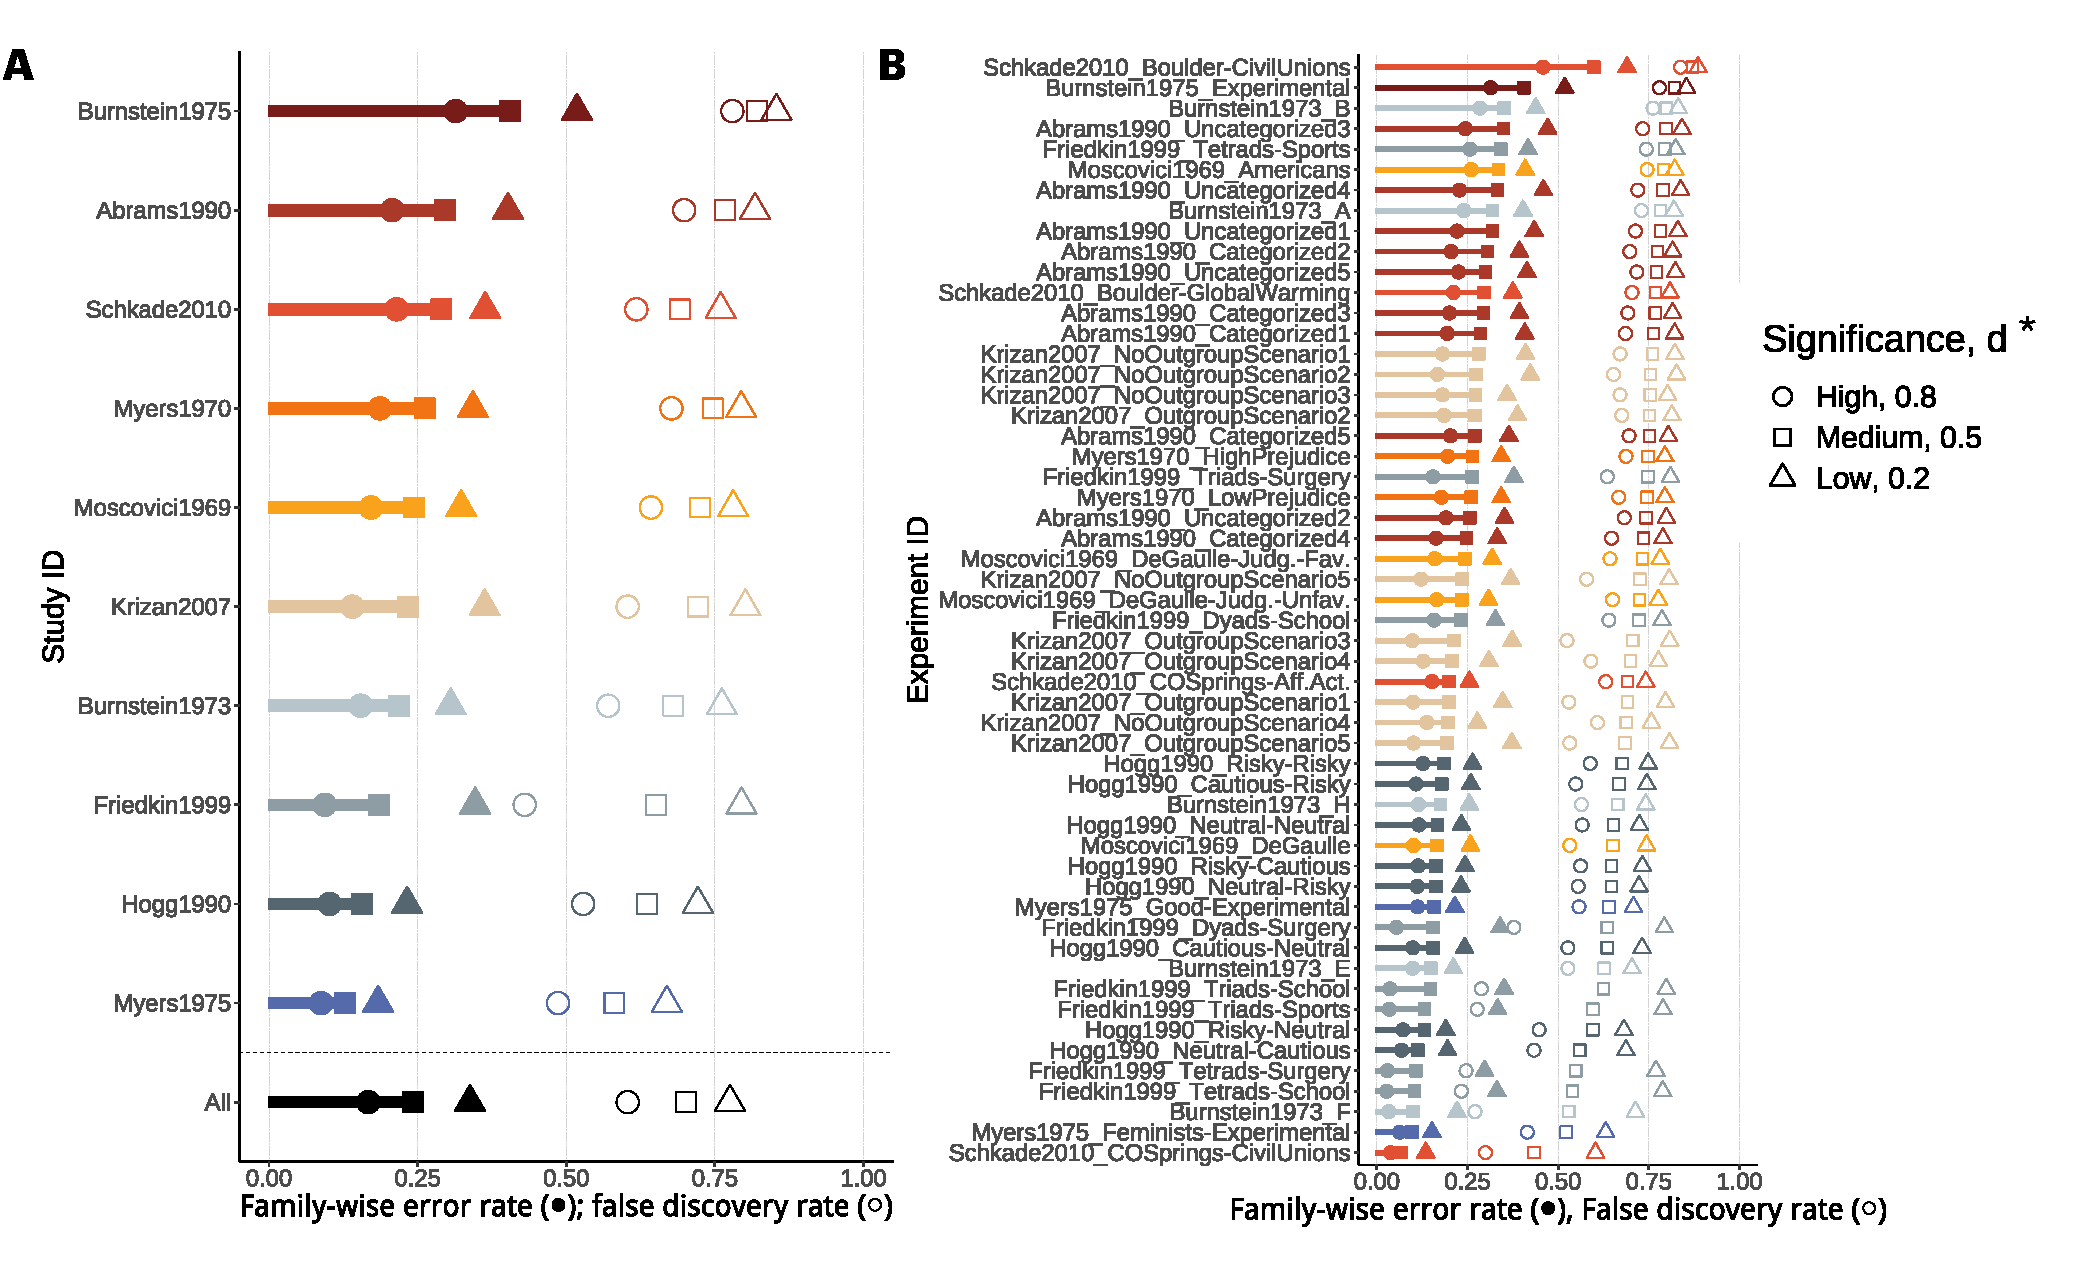
\includegraphics[width=1.1\textwidth]{Figures/Analysis/fwer_fdr_synthesis.pdf}
\end{figure} 

\begin{itemize}
  \item 
    Other $b$ and $W$ values in quantiles.
  \item
    Note that there were many ``significant'' results---in the wrong direction
    (Figure~\ref{fig:OrdinalBoxplot}).
\end{itemize}

\subsection{High significance values ($d^*$) often necessary for FWER of 0.05}

Our simulations can be used a different way, in this case to calculate what
significance value $d^*$ limits the family-wise error rate to the low value of
0.05. 
Solving the inverse problem of which $d^*$ achieves a low family-wise error rate,
which drives the false detection rate. Here we present our calculations to find
$d^*$ that achieve $\alpha(d^*) = 0.05$. 


\begin{figure}
  \caption{
    \textbf{Significance value, $d^*$, to limit family-wise error 
    rate of 0.05 for each identified study.} The Moscovici and Zavalloni (1969)
    ``Americans'' question would require the greatest $d^*$ to achieve $\alpha \leq
    0.05$, even though it does not have the highest error rates. This is because of
    larger outliers in simulated $d$ for this condition compared to others with
    greater error rates (Figure~\ref{fig:OrdinalBoxplot}).
  }
  \centering
    \includegraphics[width=0.75\textwidth]{Figures/Analysis/sigval_for_low_fwer.pdf}
  \label{fig:sigval_for_low_fwer}
\end{figure}


% \section{Discussion}\label{discussion}

\mt{Restate results and importance and outline this section.}

Since there seems to be no selection pressure on false discovery rates,
experiment design for studying group polarization was free to evolve
randomly. Various choices for the number of bins and other instrumental
details may have then become entrenched in different communities defined by
common theoretical perspectives taken by researchers in those communities.
Therefore, when Isenberg (1986)~\cite{Isenberg1986} reports that his
meta-analysis found more support for the persuasive arguments theory than the 
social comparisons theory in the form of greater effect sizes. If this were
indeed the case, perhaps it is only because some researchers hypothesizing
persuasive arguments happened to use a measurement procedure produced more
frequent and extreme distortions of opinion measurements. Incentive
structures known to promote the ``evolution of bad science'' would select
for research that ignored sticky, time-consuming statistical problems in
favor of juicy titles and headlines for which practitioners have won several
professional awards. Specifically, the traditional bias
towards positive results, and against negative ones, could easily have
provided a cultural niche in which quick but faulty group polarization
statistical methods dominate slower, more rigorous ones.
Now that we are aware of the problem, there must be
intense selective pressure applied as soon and as widely as possible to 
avoid further ``replications'' that report spurious group polarization, or
any similar latent psychological dynamics. 

We provided tools that experimenters can use. While these tools are
potentially useful, they are still in the prototype phase that was
sufficient for a single researcher who was also the software developer. So,
a first step towards expanding the usefulness of the findings here is to 
improve the software usability and make the app widely available for
researchers in group polarization and beyond. Another step would be to go
beyond reactionary testing of the reliability of experimental designs, and
identify design principles that reduce the false detection rate without
needing to adjust the Cohen's $d$ (or whatever measure) 
used as a significance threshold. 

When we used the appropriate ordered probit Bayesian statistical model, it
still often failed to accurately identify mere agreement, instead detecting
group polarization.  The ordered probit model we used still likely
underestimates the variance in outcomes, which could require even larger
sample sizes. A more rigorous analysis would include additional sources of
variance that will likely further inflate the Type I error rate, $\alpha$,
and the false discovery rate~\cite{Yarkoni2022}. First and foremost, there is
variance within each experimental deliberation group; no group polarization
study accounts for this, instead treating participants in each experimental
condition as if they were one large group. Furthermore, survey data are known
to be noisy~\cite{Zaller1992}. People report opinions differently over time
for no apparent reason (i.e., opinions are \emph{unstable}).  Context
matters: the order in which a survey question is asked, and which question
framing is chosen among logically equivalent alternatives, can both
significantly influence participant responses. Finally, little is known about
the psychological process that converts latent opinions to reporting
behaviors (e.g., clicking a radio button corresponding to an opinion).  The
effect of accounting for these sources of variance must be understood to
estimate $\alpha$ (and power, $W$) for the design of the next generation of
group polarization experiments. 

A simple change in measurement procedure could fix the problem identified
here: center the post-discussion scale on each group’s own pre-discussion
mean. This removes the assumption that all groups share a common “neutral”
midpoint. The situation is like tossing a ball on a moving train: to the
passengers, the ball’s speed is the same in both directions, but to an
observer on the ground one throw appears faster and the other slower.
Likewise, when measurement is anchored to an external scale, simple agreement
within a group can appear as movement toward one pole. Re-centering the
measurement frame corrects this distortion. It acknowledges that opinion
change is relative to the observer’s reference frame—there is no fixed
background of neutrality against which all groups can be compared. This is,
in essence, the insight of Newtonian relativity: apparent motion depends on
the frame from which it is measured.

First we must note that there are even more, perhaps even graver problems
with group polarization research than I discussed so far: one of note is
opinion instability. Opinions are not generally stable—people seem to
construct their opinions based on several factors not directly related to
whatever underlying topic. Factors affecting reported opinions include the
language used to frame a prompt or question; the order of questions on a
multi-item survey; or simply when the question was asked (Kalton and Schuman,
1982; Zaller and Feldman, 1992; Zaller 1992). Failure to account for sources
of input variance in any experiment can lead to inflated effect sizes since
the input variance is missing from the posterior predictions during
statistical model fitting (Yarkoni, 2022). This further compounds the
theoretical confusions that fill the void when theories are never formalized
and grounded in a mathematical or computational model (Smaldino 2020; Turner
and Smaldino, 2022).

A second additional problem with group polarization research is that we literally cannot learn anything by comparing summary statistics obtained with incommensurate experimental designs—but this is exactly how group polarization research has tried to make progress. Comparing summary statistics only has explanatory power if datasets were generated under the same experimental designs—it seems this was never done or even considered in the group polarization literature. In order to compare studies, their datasets must be generated from commensurate experiments, meaning the studies must share the same predictive and statistical models and experimental design. Otherwise, such comparisons are meaningless, they literally tell us nothing, as shown by philosopher of science Nancy Cartwright in Chapter 5 of her book The Dappled World: A Study of the Boundaries of Science.


\subsection{Humble Hearts Promote Rigorous Science}

Cass Sunstein kicked off the 2000s by elevating group polarization to be a scientific law and advocating the application of group polarization research to serious real-world problems in two books (Sunstein, 2009; Sunstein, 2019) and two recent high-profile articles in Nature Human Behavior: one on the social foundations of pandemic preparedness (Van Bavel, et al., 2020) and one to “promote truth, autonomy, and democratic discourse online” (Lorenz-Spreen, Lewandowski, Sunstein, and Hertwig, 2020). Let us try to stop the spread of this bad science—and let us explore what must be done to achieve Dorian Cartwright’s vision of a rigorous science of group polarization he articulated fifty years ago.

To be practically useful, science must be rigorous. Rigorous science comes most naturally when scientists remain humble, especially when they serve at the pleasure of the public, the government, or other donors. Here’s another example from Burnstein and Vinokur (1973) that we can learn from—let’s try to avoid the sort of arrogance and haughtiness that seep from these acknowledgements they wrote on p. 123:

\begin{quote}
This research was supported by a Grant from the National Institute of Mental Health (MH-16950-03) and by a Guggenheim Foundation Fellowship awarded to the first author. We gratefully acknowledge the incisive, witty, and vinous commentary provided by colleagues at the University of Provence, in particular Robert Abelson, Claude Flament, and Jean-Pierre Poitou, as well as the spirited and intelligent efforts of Livia Mezrick and Irene Graczyk, who helped us carry out the study.
\end{quote}

Science is not glamorous—it takes guts and sacrifice to achieve the technical skills and discipline to sharpen one’s prose, methods, mathematics, and computer code to the point they can really cut reality at its joints, investigate different parts, then put it all back together with a message for others about how the world really works. These days, to do rigorous social science work one must wisely curate the best of the available social science by harmonizing cross-disciplinary jargon. But disincentives still exist against careful scholarship. Prizes and professorships go to those with the most numerous publications in the right journals—period.

Unpaid, anonymous reviewers are supposed to act as gatekeepers to catch problems like the ones I reviewed. But, journal article reviewers have little to gain from enforcing rigor—actually there is a lazy strategy that can pay off big for freeloaders. It’s easy to imagine a cultural norm evolving where reviewers save themselves time and energy by asking little of an author, in hopes that little will be demanded of them when the reviewer submits their next paper. This could result in a publication process that rewards the laziest and most willing to flood the zone and self-aggrandize.

\subsection{Conclusion}

Social science can use physics as a model discipline to transition from idiosyncratic and Balkanized to informative and united. Physics only changed the world because it is useful—it is useful only because it reliably predicts things. Physics became more useful as it became more united, finding shared representations for concepts developed independently—for example the science of optics was developed independently from the science of dynamics, but the physics of light is explained partly in analogy to a pendulum or spring—the mathematics of harmonic motion can be used to predict the motion of springs or pendulums—or why we see different colors of light through a prism. With careful, coordinated tweaks to group polarization experimental design and theoretical modeling, we will build a more rigorous theory of group polarization and its large-scale expression, echo chamber radicalization.

I expect that group polarization experiments, when properly constructed and analyzed, will help sustainability campaigns optimize their social influence campaigns. We can start by developing simpler experimental designs based on formal or computational models capable of predicting outcomes in an experiment. I have developed a model that could motivate an experimental design: I showed that if extremists are more stubborn, this is sufficient to cause group polarization when likeminded groups interact over time. There is even a free stubborn extremism parameter that could be fit to data to measure the relationship between stubbornness and extremism on different issues.

Group polarization research so far has mostly provided us with a checklist of what not to do. The alternative approach I outline builds on rock—the rock of rigor—and will supersede past group polarization research built on a thousand grains of inexact verbal speculation.


\section{Discussion}\label{discussion}

\mt{Restate results and importance and outline this section.}

Since there seems to be no selection pressure on false discovery rates,
experiment design for studying group polarization was free to evolve
randomly. Various choices for the number of bins and other instrumental
details may have then become entrenched in different communities defined by
common theoretical perspectives taken by researchers in those communities.
Therefore, when Isenberg (1986)~\cite{Isenberg1986} reports that his
meta-analysis found more support for the persuasive arguments theory than the 
social comparisons theory in the form of greater effect sizes. If this were
indeed the case, perhaps it is only because some researchers hypothesizing
persuasive arguments happened to use a measurement procedure produced more
frequent and extreme distortions of opinion measurements. Incentive
structures known to promote the ``evolution of bad science'' would select
for research that ignored sticky, time-consuming statistical problems in
favor of juicy titles and headlines for which practitioners have won several
professional awards. Specifically, the traditional bias
towards positive results, and against negative ones, could easily have
provided a cultural niche in which quick but faulty group polarization
statistical methods dominate slower, more rigorous ones.
Now that we are aware of the problem, there must be
intense selective pressure applied as soon and as widely as possible to 
avoid further ``replications'' that report spurious group polarization, or
any similar latent psychological dynamics. 

We provided tools that experimenters can use. While these tools are
potentially useful, they are still in the prototype phase that was
sufficient for a single researcher who was also the software developer. So,
a first step towards expanding the usefulness of the findings here is to 
improve the software usability and make the app widely available for
researchers in group polarization and beyond. Another step would be to go
beyond reactionary testing of the reliability of experimental designs, and
identify design principles that reduce the false detection rate without
needing to adjust the Cohen's $d$ (or whatever measure) 
used as a significance threshold. 

When we used the appropriate ordered probit Bayesian statistical model, it
still often failed to accurately identify mere agreement, instead detecting
group polarization.  The ordered probit model we used still likely
underestimates the variance in outcomes, which could require even larger
sample sizes. A more rigorous analysis would include additional sources of
variance that will likely further inflate the Type I error rate, $\alpha$,
and the false discovery rate~\cite{Yarkoni2022}. First and foremost, there is
variance within each experimental deliberation group; no group polarization
study accounts for this, instead treating participants in each experimental
condition as if they were one large group. Furthermore, survey data are known
to be noisy~\cite{Zaller1992}. People report opinions differently over time
for no apparent reason (i.e., opinions are \emph{unstable}).  Context
matters: the order in which a survey question is asked, and which question
framing is chosen among logically equivalent alternatives, can both
significantly influence participant responses. Finally, little is known about
the psychological process that converts latent opinions to reporting
behaviors (e.g., clicking a radio button corresponding to an opinion).  The
effect of accounting for these sources of variance must be understood to
estimate $\alpha$ (and power, $W$) for the design of the next generation of
group polarization experiments. 

A simple change in measurement procedure could fix the problem identified
here: center the post-discussion scale on each group’s own pre-discussion
mean. This removes the assumption that all groups share a common “neutral”
midpoint. The situation is like tossing a ball on a moving train: to the
passengers, the ball’s speed is the same in both directions, but to an
observer on the ground one throw appears faster and the other slower.
Likewise, when measurement is anchored to an external scale, simple agreement
within a group can appear as movement toward one pole. Re-centering the
measurement frame corrects this distortion. It acknowledges that opinion
change is relative to the observer’s reference frame—there is no fixed
background of neutrality against which all groups can be compared. This is,
in essence, the insight of Newtonian relativity: apparent motion depends on
the frame from which it is measured.

First we must note that there are even more, perhaps even graver problems
with group polarization research than I discussed so far: one of note is
opinion instability. Opinions are not generally stable—people seem to
construct their opinions based on several factors not directly related to
whatever underlying topic. Factors affecting reported opinions include the
language used to frame a prompt or question; the order of questions on a
multi-item survey; or simply when the question was asked (Kalton and Schuman,
1982; Zaller and Feldman, 1992; Zaller 1992). Failure to account for sources
of input variance in any experiment can lead to inflated effect sizes since
the input variance is missing from the posterior predictions during
statistical model fitting (Yarkoni, 2022). This further compounds the
theoretical confusions that fill the void when theories are never formalized
and grounded in a mathematical or computational model (Smaldino 2020; Turner
and Smaldino, 2022).

A second additional problem with group polarization research is that we literally cannot learn anything by comparing summary statistics obtained with incommensurate experimental designs—but this is exactly how group polarization research has tried to make progress. Comparing summary statistics only has explanatory power if datasets were generated under the same experimental designs—it seems this was never done or even considered in the group polarization literature. In order to compare studies, their datasets must be generated from commensurate experiments, meaning the studies must share the same predictive and statistical models and experimental design. Otherwise, such comparisons are meaningless, they literally tell us nothing, as shown by philosopher of science Nancy Cartwright in Chapter 5 of her book The Dappled World: A Study of the Boundaries of Science.

\subsection{The Full Bayesian Rigor: Deriving Effect Size Posteriors and Justifying the FPR Approximation}

In evaluating the \textbf{False Positive Rate (FPR)} of a simulated null model, the primary challenge is moving beyond the raw parameter posterior distributions ($p(\mu_1 | \text{data})$, $p(\sigma_2 | \text{data})$, etc.) to accurately quantify the posterior distribution of the derived \textbf{effect size}, $d$. This section outlines the statistically rigorous method for this derivation and justifies the pragmatic approximation necessary for the evaluation stage of this paper.

\subsubsection{The most rigorous formulation of $d$}

In our model, the effect size $d$ is a function of four estimated parameters ($\mu_1, \mu_2, \sigma_1, \sigma_2$), defined by the authors whose work we replicate as:

\begin{equation}
d = \frac{\mu_1 - \mu_2}{\sqrt{(\sigma_1^2 + \sigma_2^2)/2}}
\end{equation}

The statistically rigorous method for obtaining the posterior distribution of $d$, denoted $p(d | \text{data})$, is through \textbf{marginalization by sampling} across the joint posterior distribution of the primary parameters $p(\mu_1, \mu_2, \sigma_1, \sigma_2 | \text{data})$.

\paragraph{Necessity of MCMC Samples}

The parameters are fundamentally \textbf{sequentially dependent} in the MCMC chain, as the estimation of means is conditional on the estimation of variances. This dependency is captured in the \textbf{joint posterior distribution}.

To maintain statistical rigor, we must avoid calculating $d$ by combining the isolated summary statistics (e.g., the posterior median of $\mu_1$ and the posterior median of $\sigma_1$) because this procedure, known as \textbf{plug-in estimation}, ignores the critical correlation between parameters, resulting in an unquantified and likely underestimated uncertainty.

The correct procedure requires using the full MCMC samples:

\begin{enumerate}
    \item For each usable iteration $k$ of the Markov Chain (where $K$ is the total number of samples), a plausible set of values is drawn: $(\mu_1^{(k)}, \mu_2^{(k)}, \sigma_1^{(k)}, \sigma_2^{(k)})$.
    \item The effect size is calculated for that specific set of values:
    $$d^{(k)} = \frac{\mu_1^{(k)} - \mu_2^{(k)}}{\sqrt{\frac{(\sigma_1^{(k)})^2 + (\sigma_2^{(k)})^2}{2}}}$$
    \item The set $\{d^{(1)}, d^{(2)}, \ldots, d^{(K)}\}$ then forms the complete posterior distribution $p(d | \text{data})$.
\end{enumerate}

The center of this distribution, the \textbf{posterior median} ($\tilde{d}$), is the most robust point estimate for the effect size, as it minimizes expected absolute error and is less sensitive to potential skewness than the posterior mean.

\subsubsection{Justifying the FPR Approximation}

Due to the computational complexity and the unavailability of the original MCMC chains for all $57,000$ fits, a pragmatic simplification was necessary for the subsequent evaluation of the False Positive Rate (FPR).

\paragraph{The FPR Criterion}

A standard method for estimating the FPR (or Type I error rate) in simulation studies is to count the proportion of null trials where the observed effect size meets or exceeds a predefined threshold, $d^*$.

$$\text{FPR} = \frac{\text{Number of Null Fits where } |d| > d^*_{\text{threshold}}}{\text{Total Number of Null Simulations}}$$

In this analysis, $d^*_{\text{threshold}}$ is set to the commonly adopted small effect size threshold of $d^*=0.2$ (and varied for sensitivity analysis), avoiding the reliance on approximated $95\%$ credible intervals, which would require further, less reliable approximations.

\paragraph{The Compromise: Plug-in and Heuristics}

We employed a simplified plug-in value for $d$ using the stored posterior means:

$$d_{\text{plug}} = \frac{\hat{\mu}_1 - \hat{\mu}_2}{\sqrt{(\hat{\sigma}_1^2 + \hat{\sigma}_2^2)/2}}$$

Where $\hat{\theta}$ represents the \textbf{posterior mean} of the parameter $\theta$.

While this approach is a statistical shortcut, the error is mitigated by two factors: the use of the $d^*_{\text{threshold}}$ heuristic, and the large simulated sample size ($N=500$ per group), which ensures that the posteriors for $\mu$ and $\sigma$ are sufficiently narrow. This minimizes the difference between $d_{\text{plug}}$ and the true posterior median $\tilde{d}$, making the shortcut defensible as a pragmatic necessity given the study's scale.

\subsection{Humble Hearts Promote Rigorous Science}

Cass Sunstein kicked off the 2000s by elevating group polarization to be a scientific law and advocating the application of group polarization research to serious real-world problems in two books (Sunstein, 2009; Sunstein, 2019) and two recent high-profile articles in Nature Human Behavior: one on the social foundations of pandemic preparedness (Van Bavel, et al., 2020) and one to “promote truth, autonomy, and democratic discourse online” (Lorenz-Spreen, Lewandowski, Sunstein, and Hertwig, 2020). Let us try to stop the spread of this bad science—and let us explore what must be done to achieve Dorian Cartwright’s vision of a rigorous science of group polarization he articulated fifty years ago.

To be practically useful, science must be rigorous. Rigorous science comes most naturally when scientists remain humble, especially when they serve at the pleasure of the public, the government, or other donors. Here’s another example from Burnstein and Vinokur (1973) that we can learn from—let’s try to avoid the sort of arrogance and haughtiness that seep from these acknowledgements they wrote on p. 123:

\begin{quote}
This research was supported by a Grant from the National Institute of Mental Health (MH-16950-03) and by a Guggenheim Foundation Fellowship awarded to the first author. We gratefully acknowledge the incisive, witty, and vinous commentary provided by colleagues at the University of Provence, in particular Robert Abelson, Claude Flament, and Jean-Pierre Poitou, as well as the spirited and intelligent efforts of Livia Mezrick and Irene Graczyk, who helped us carry out the study.
\end{quote}

Science is not glamorous—it takes guts and sacrifice to achieve the technical skills and discipline to sharpen one’s prose, methods, mathematics, and computer code to the point they can really cut reality at its joints, investigate different parts, then put it all back together with a message for others about how the world really works. These days, to do rigorous social science work one must wisely curate the best of the available social science by harmonizing cross-disciplinary jargon. But disincentives still exist against careful scholarship. Prizes and professorships go to those with the most numerous publications in the right journals—period.

Unpaid, anonymous reviewers are supposed to act as gatekeepers to catch problems like the ones I reviewed. But, journal article reviewers have little to gain from enforcing rigor—actually there is a lazy strategy that can pay off big for freeloaders. It’s easy to imagine a cultural norm evolving where reviewers save themselves time and energy by asking little of an author, in hopes that little will be demanded of them when the reviewer submits their next paper. This could result in a publication process that rewards the laziest and most willing to flood the zone and self-aggrandize.

\subsection{Conclusion}

Social science can use physics as a model discipline to transition from idiosyncratic and Balkanized to informative and united. Physics only changed the world because it is useful—it is useful only because it reliably predicts things. Physics became more useful as it became more united, finding shared representations for concepts developed independently—for example the science of optics was developed independently from the science of dynamics, but the physics of light is explained partly in analogy to a pendulum or spring—the mathematics of harmonic motion can be used to predict the motion of springs or pendulums—or why we see different colors of light through a prism. With careful, coordinated tweaks to group polarization experimental design and theoretical modeling, we will build a more rigorous theory of group polarization and its large-scale expression, echo chamber radicalization.

I expect that group polarization experiments, when properly constructed and analyzed, will help sustainability campaigns optimize their social influence campaigns. We can start by developing simpler experimental designs based on formal or computational models capable of predicting outcomes in an experiment. I have developed a model that could motivate an experimental design: I showed that if extremists are more stubborn, this is sufficient to cause group polarization when likeminded groups interact over time. There is even a free stubborn extremism parameter that could be fit to data to measure the relationship between stubbornness and extremism on different issues.

Group polarization research so far has mostly provided us with a checklist of what not to do. The alternative approach I outline builds on rock—the rock of rigor—and will supersede past group polarization research built on a thousand grains of inexact verbal speculation.


\section*{Tables}

\begin{table}[ht]
\centering
\caption{\textbf{Journal articles in our corpus.}}
\label{tab:articles}

\begin{tabular}{m{0.9in} m{1.35in} m{2.45in} m{1.3in}}
\toprule
\textbf{Category} & \textbf{Authors (Year)} & \textbf{Title} & \textbf{Journal} \\
\midrule

\rowcolor{gray!5}
\multirowcell{2}{Politics} 
                  & Moscovici \& Zavalloni (1969)~\cite{Moscovici1969} & The Group as a Polarizer of Attitudes & \emph{JPSP} \\
\rowcolor{gray!5}
                  & Schkade, Sunstein, \& Hastie (2010)~\cite{Schkade2010} & When Deliberation Produces Extremism & \emph{Critical~Review} \\[0.2em]

\multirowcell{2}{Social Comp's \vspace{0.7em}}
% \multirowcell{2}{Social Comp's}
                  & Myers \& Bishop (1970)~\cite{Myers1970} & Discussion Effects on Racial Attitudes & \emph{Science} \\[0.2em]
                  & Myers (1975)~\cite{Myers1975} & Discussion-Induced Attitude Polarization & \emph{Human Relations} \\[0.3em]

\rowcolor{gray!5}
\multirowcell{2}{Persuasive Arg's}
                  & Burnstein \& Vinokur (1973)~\cite{Burnstein1973} & Testing Two Classes of Theories About Group Induced Shifts In Individual Choice & \emph{JESP} \\
\rowcolor{gray!5}
                  & Burnstein \& Vinokur (1975)~\cite{Burnstein1975} & What a person thinks upon learning he has chosen differently from others: Nice evidence for the persuasive-arguments\ldots & \emph{JESP} \\

\multirowcell{3}{Self-Categ'n}
                  & Abrams, et al., (1990)~\cite{Abrams1990} & Knowing What to Think by Knowing Who You Are: Self‐Categorization and the Nature of Norm Formation\ldots & \emph{Brit. J. of Soc. Psy.} \\
                  & Hogg, Turner, \& Davidson (1990)~\cite{Hogg1990} & Polarized Norms and Social Frames of Reference: A Test of the Self-Categorization Theory of Group Polarization & \emph{B. \& Appl. Soc. Psy.} \\
                  & Krizan \& Baron (2007)~\cite{Krizan2007} & Group Polarization and Choice Dilemmas: How Important is Self-Categorization? & \emph{Eur. J. of Soc. Psy.} \\

\rowcolor{gray!5}
\multirowcell{1}{Soc'l Decisions}
                  & Friedkin (1999)~\cite{Friedkin1999} & Choice Shifts \& Group Polarization & \emph{Amer. Soc. Rev.} \\

\bottomrule
\end{tabular}
\end{table}


%%%%%%%%%%%%%%%%%%%
% TABLES OF VARIABLES IN METHOD
\begin{table}[h]
  \caption{\textbf{Latent psychological variables and distributions.}}
  \label{tab:latent-variables}
  \begin{tabular}{cll} 
  \toprule
    \textbf{Variable} & \textbf{Description} & \textbf{Values} \\
  \midrule  
    $\omega_{i,t}$ & Latent opinion of individual $i$ at time $t$ & $\mathbb{R}$ \\
    $\mu_t$ & Mean latent opinion at time $t$ (constant in null-polarization) & $\mathbb{R}$ \\
    $\sigma_t$ & Variance of observed opnions at time $t$ & $\mathbb{R}$ \\
  \bottomrule
  \end{tabular} 
\end{table}

\begin{table}[h]
  \caption{\textbf{Experimental design and numerical model parameters.}}
  \label{tab:experiment-parameters}
  \begin{tabular}{cll} 
  \toprule
    \textbf{Variable} & \textbf{Description} & \textbf{Values} \\
  \midrule  
    $B$ & Number of bins & $5,6,7,\ldots$ \\
    $\theta_b$ & The $B+1$ threshold values that separate bins & 
      e.g., $-\infty, -2.5, -1.5,\ldots,2.5, \infty$ \\
    $b$ & Bin index—there are $B+1$ to mark $B$ bins & $0,1,2,\ldots,B$ \\
  \bottomrule
  \end{tabular} 
\end{table}

\begin{table}[h]
  \caption{\textbf{Simulated observed variables.}}
  \label{tab:simulated-observations}
  \begin{tabular}{cll} 
  \toprule
    \textbf{Variable} & \textbf{Description} & \textbf{Values} \\
  \midrule  
    $\meanobst$ & Mean of all reported opinions (Equation \ref{eq:meanobs}) & $\mathbb{R}$ \\
    $g(\nu)$ & Spurious group opinion polarization for null-polarization params $\nu$
    (Equation \ref{eq:group-polarization})
        & $\mathbb{R}$ \\
    $d_{ei}$ & Cohen's $d$ for the $i^{\mathrm{th}}$ simulation of experiment $e$ & $\mathbb{R}$ \\
    $d*$ & Significance value in terms of Cohen's $d$, e.g., $d^* \geq 0.5$ as a
    "medium" effect\footnote{According to Cohen (1986)\cite{CohenBook1988}.} & $\mathbb{R}$ \\
    $\alpha_e,\alpha_s,\alpha_{\text{all}}$ & False positive rate
    for an experiment, $e$; study, $s$; or across \emph{all} experiments.
             & $[0, 1]$ \\
    FDR$_e$ & False detection rate: calculated using $\alpha_e$ to get chance experimental
    detection is false\footnote{See Equation~\ref{eq:fdr}}
        & $[0, 1]$ \\
  \bottomrule
  \end{tabular} 
\end{table}

\section*{Figures}

\begin{figure}[ht]
  \caption{\textbf{Opinion measurement model and spurious group polarization.} 
  Latent model participant opinions are drawn from a normal distribution with the
  listed parameters (A,C). The pre-deliberation latent distribution has high
  variance, but appears polarized when measured via integration (A).  The latent
  distribution's variance is expected to decrease during deliberation (B) via
  consensus, but in this example the latent mean is static, 
$\mupre = \mupost$. However, when the post-deliberation distribution is measured,
the simulated observed mean increases, i.e., spurious
group polarization occurs (C).}
  \centering
  \includegraphics[width=0.95\textwidth]{Figures/Model/latent-ordinal-distros.pdf}
  \label{fig:distros}
\end{figure}





\clearpage

\printbibliography[title=References]

\appendix

\renewcommand{\thefigure}{A\arabic{figure}}
\setcounter{figure}{0}
\clearpage

%%%%%%%%%% Supplement %%%%%%%%%%
\pagebreak
\begin{center}
  \textbf{\Large \textsf{Group polarization replications may be marred by high false discovery rates (Supplementary Material)}}
\end{center}

%%%%%%%%%% Prefix a "S" to all equations, figures, tables and reset the counter %%%%%%%%%%
\setcounter{equation}{1}
\setcounter{figure}{0}
\setcounter{section}{0}
\setcounter{table}{0}
\setcounter{page}{1}
\makeatletter
\renewcommand{\theequation}{S\arabic{equation}}
\renewcommand{\thefigure}{S\arabic{figure}}
\renewcommand{\thetable}{S\arabic{table}}
\renewcommand{\thesection}{S\arabic{section}}
\renewcommand{\thepage}{S\arabic{page}}
\makeatother

\section{Supplemental Analyses}

\begin{figure}
  \caption{Boxplot of Cohen's $d$ for the ordered probit model over 1000
    simulation trials for each experimental condition (y-axis in A and B).
    Each trial represents a possible outcome of a group polarization experiment where
    the true opinion shift is zero. The mean across trials is closer to 0 than
    in the metric case, but many simulated zero-shift experiments still result in
    an observed shift. This illustrates the weak statistical power of these group
    polarization experiments.}
  \label{fig:OrdinalBoxplot}
  \centering
    \includegraphics[width=1.0\textwidth]{Figures/Analysis/ordinal_cohens.pdf}
\end{figure}

\end{document}
